%!TEX root = report.tex

\chapter{Appendix}
\label{appendix}

  \section{Demonstrations} % (fold)
  \label{sec:demonstrations}
  
    Two demonstrations of the developed prototype can be seen in:

    \url{https://raw.githubusercontent.com/carsy/rama-spotify/master/demo.gif} \\
    and \\
    \indent \url{https://raw.githubusercontent.com/carsy/rama-spotify/master/demo2.gif} \\

    An effort was made to show the main implemented features.
    

  % section demonstrations (end)

  \section{Questionnaire} % (fold)
  \label{sec:questionnaire}

    The questionnaire in Figure~\ref{fig:questionnaire} was composed of four mandatory questions and a free-text field for suggestions and other feedback.
  
    \begin{figure}
      \begin{center}
        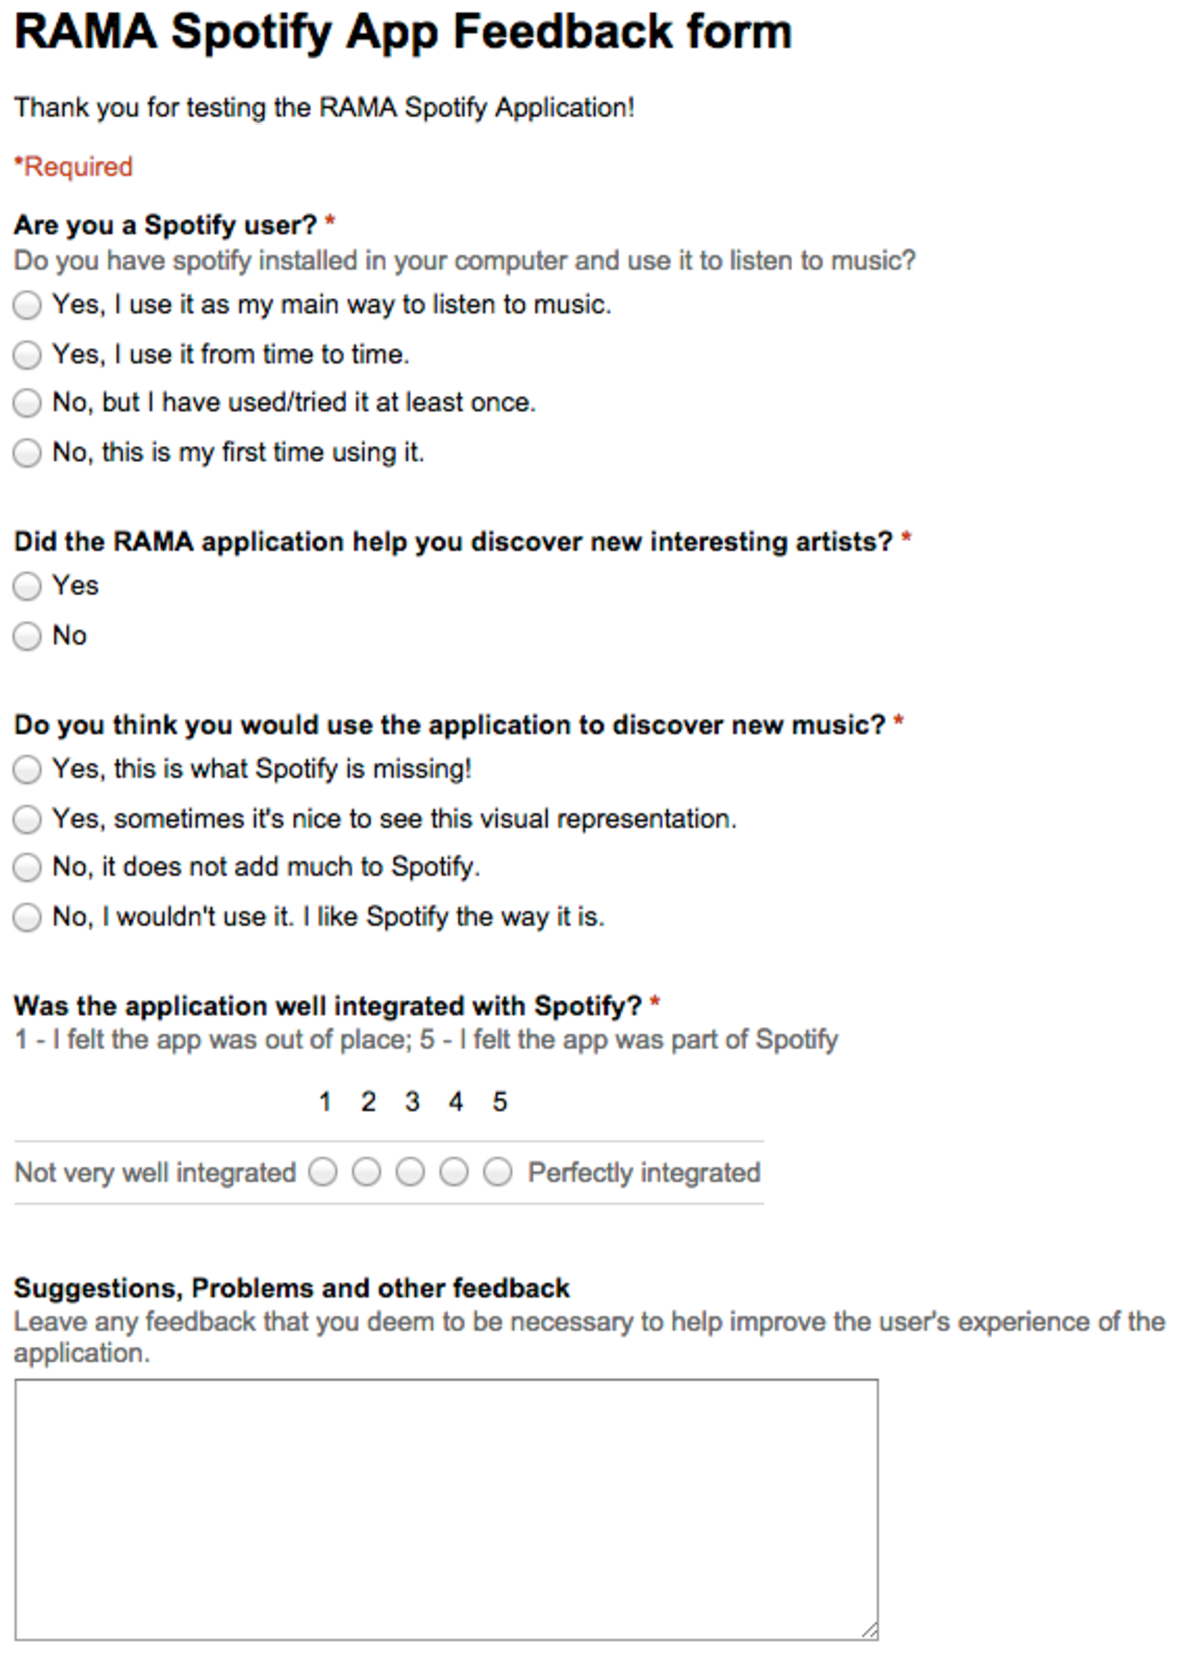
\includegraphics[width=\textwidth]{questionnaire.pdf}
      \end{center}
      \caption{Questionnaire that the beta-testers were required to fill after the experiment.}
      \label{fig:questionnaire}
    \end{figure}
  
  % section questionnaire (end)

  \section{Submissions} % (fold)
  \label{sec:submissions}
  
    Two submissions will be sent to the following conferences:

    \begin{itemize}
      \item ISMIR 2014\footnote{\url{http://www.terasoft.com.tw/conf/ismir2014}} - Demo submission\footnote{\url{http://www.terasoft.com.tw/conf/ismir2014/theLBD.html}}
      \item INFORUM 2014\footnote{\url{http://inforum.org.pt/INForum2014}} - Comunication and poster\footnote{\url{http://inforum.org.pt/INForum2014/submissoes}}
    \end{itemize}

  % section submissions (end)

  

  % NOTE
  % add important code snippets.